\documentclass{beamer}
\mode<presentation>
{
  \usetheme{ldv}
  \setbeamercovered{transparent}
}

% Uncomment this if you're giving a presentation in german...
\usepackage[ngerman]{babel}

% ...and rename this to "Folie"
\newcommand{\slidenomenclature}{Folie}


\usepackage[utf8]{inputenc}
\usepackage{amsmath,amssymb,amsfonts}
\usepackage{times}
\usepackage{graphicx}
\usepackage{fancyvrb}
\usepackage{array}
\usepackage{colortbl}
\usepackage{tabularx}

% Uncomment me when you need to insert code
\usepackage{color}
\usepackage{listings}
\usepackage{minted}
\usepackage{algpseudocode}
% End Code

\usepackage{datetime}
\usepackage{tikz}

\usetikzlibrary{calc}
\usetikzlibrary{shapes.geometric}
\usetikzlibrary{decorations.pathreplacing}
\usetikzlibrary{positioning}

% Uncomment me when you need video or sound
% \usepackage{multimedia}
% \usepackage{hyperref}
% End video

% Header
\newcommand{\zwischentitel}{Woche 8}
\newcommand{\leitthema}{Tobias Eppacher}
\newcommand{\presdatum}{\formatdate{16}{6}{2025}}
% End Header

% Titlepage
\title{Grundlagen: Algorithmen und Datenstrukturen}
\author{Tobias Eppacher}
\date{\presdatum}
\institute{School of Computation, Information and Technology}
\subtitle{Woche 8}
% End Titlepage


% Slides
\begin{document}


% 1. Slide: Titlepage
\begin{frame}
	\titlepage
\end{frame}

% 2. Slide: TOC
\begin{frame}
	\frametitle{Inhalt}
	\tableofcontents[subsectionstyle=hide]
\end{frame}

\section{Aufgaben}
\begin{frame}
	\frametitle{Aufgabe 8.1 - Binomialheaps}

	{\footnotesize
		Führen Sie auf dem folgenden Binomial-Heap nacheinander drei deleteMin-Operationen aus.
		Fügen Sie anschließend die drei entfernten Elemente in der Reihenfolge, in der sie entfernt
		wurden, wieder hinzu. Zeichnen Sie nach jeder deleteMin- und insert-Operation den entstandenen Binomial-Heap.
		Sind nach allen Operationen die Werte an derselben Stelle im Heap?
		Hat der Heap nach allen Operationen dieselbe Struktur? Warum?
	}

	\medskip

	\begin{center}
		\begin{tikzpicture}[nodeStyle/.style={circle, draw, minimum size=0.8cm}, scale=0.7, transform shape]
			% Roots
			\node[nodeStyle] (3) at (0, 0) {3};
			\node[nodeStyle] (5) at (3, 0) {5};

			% Layer 1
			\node[nodeStyle] (4) at (-3, -1.5) {4};
			\node[nodeStyle] (7) at (-1.5, -1.5) {7};
			\node[nodeStyle] (6) at (0 , -1.5) {6};

			% Layer 2
			\node[nodeStyle] (9) at (-4.5, -3) {9};
			\node[nodeStyle] (11) at (-3, -3) {11};

			\node[nodeStyle] (8) at (-1.5, -3) {8};

			% Layer 3
			\node[nodeStyle] (10) at (-4.5, -4.5) {10};

			\draw (3) -- (4);
			\draw (3) -- (7);
			\draw (3) -- (6);
			\draw (4) -- (9);
			\draw (4) -- (11);
			\draw (7) -- (8);
			\draw (9) -- (10);

			\draw[dashed, <-] (3.east) -- (5.west);

			\node[above=0.4cm of 3] (min_label) {min};
			\draw[red, ->] (min_label.south) -- (3.north);

		\end{tikzpicture}
	\end{center}
\end{frame}

\begin{frame}[t]
	\frametitle{Aufgabe 8.1 -  Binomialheaps}
	Erste Operation:
\end{frame}

\begin{frame}[t]
	\frametitle{Aufgabe 8.1 -  Binomialheaps}
	Zweite Operation:
\end{frame}

\begin{frame}[t]
	\frametitle{Aufgabe 8.1 -  Binomialheaps}
	Dritte Operation:
\end{frame}

\begin{frame}[t]
	\frametitle{Aufgabe 8.1 -  Binomialheaps}
	Vierte Operation (ab hier Variante 1):
\end{frame}

\begin{frame}[t]
	\frametitle{Aufgabe 8.1 -  Binomialheaps}
	Fünfte Operation:
\end{frame}

\begin{frame}[t]
	\frametitle{Aufgabe 8.1 -  Binomialheaps}
	Sechste Operation:
\end{frame}

\begin{frame}[t]
	\frametitle{Aufgabe 8.2 - Rückblick: Circular Queues (a)}
	{\small
		Gegeben sei ein Zirkulärer Ringspeicher als FIFO-Queue. In folgenden Darstellungen
		wird der Head mit \textbf{H} und der Tail mit \textbf{T} markiert. Geben Sie an, wie viele Inserts in
		folgenden Queues noch möglich sind. Dabei sollen Elemente, die aktuell in der Queue
		sind, weder überschrieben noch entfernt werden:
	}

	\medskip

	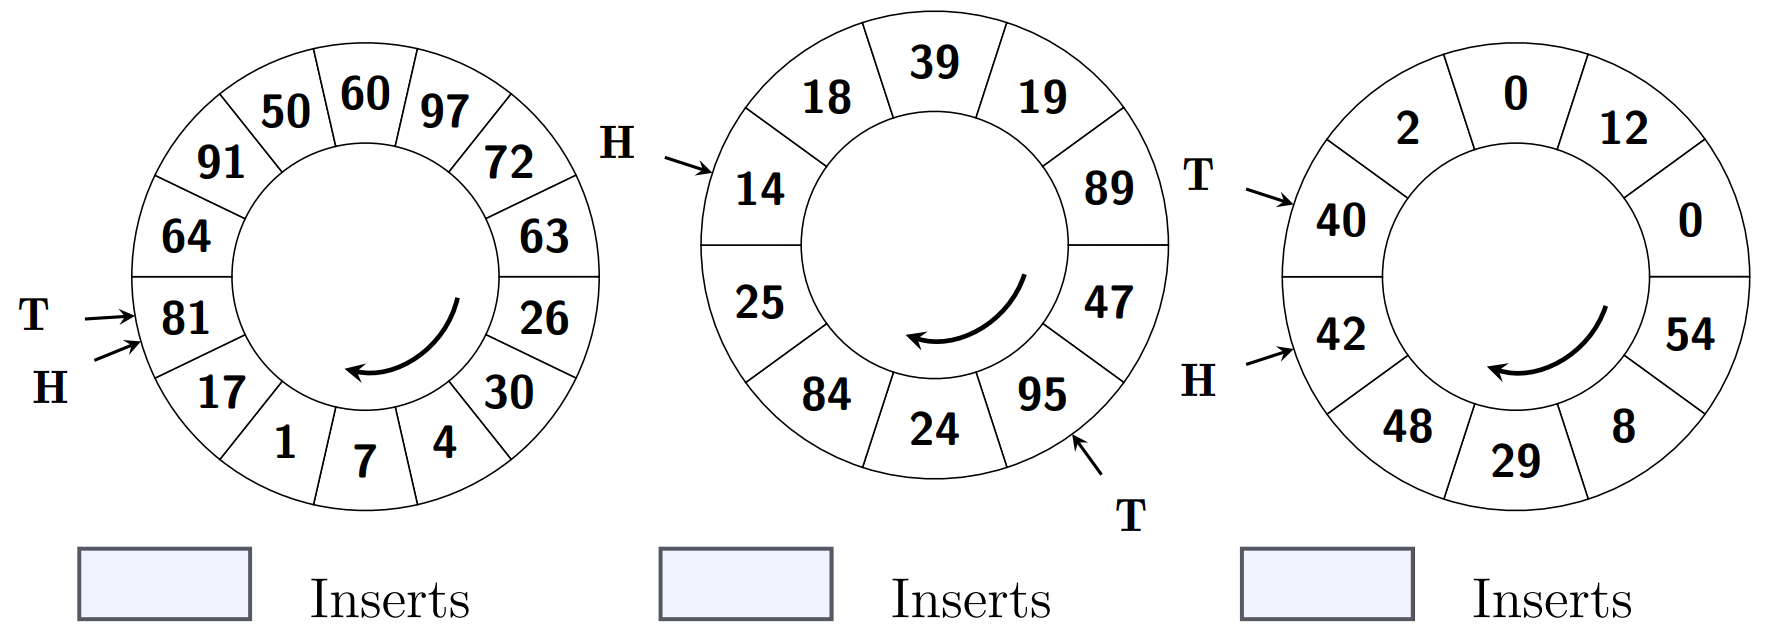
\includegraphics[width=\textwidth]{images/circular_queue_a.png}
\end{frame}

\begin{frame}[t]
	\frametitle{Aufgabe 8.2 - Rückblick: Circular Queues (b)}
	{\small
		Der folgende Ringspeicher wird nun als \textbf{Deque} genutzt. Geben Sie den Ringspeicher
		an, nachdem folgende Operationen ausgeführt wurden: \textbf{pushFront(23), pushBack(42),
			popFront()}
	}

	\medskip

	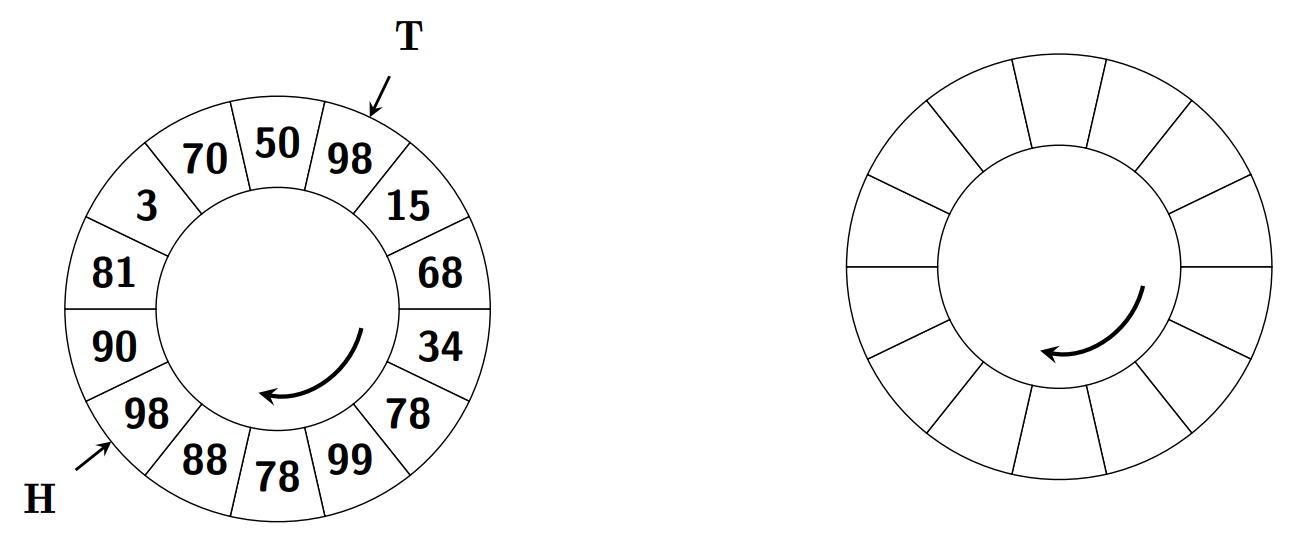
\includegraphics[width=\textwidth]{images/circular_queue_b.png}
\end{frame}

\begin{frame}[t]
	\frametitle{Aufgabe 8.3 - Rückblick: Landausymbole (a)}
	Gegeben seien die Funktionen $f$, $g$ mit $f(n) = \log_2{n} \ast g(n)$. Begründen Sie folgende
	Aussagen oder widerlegen Sie sie mit einem Gegenbeispiel:

	\begin{enumerate}
		\setlength{\itemsep}{6em}
		\item Aus $g = \mathcal{O}(n)\ $ folgt $\ f = \mathcal{O}(\log_2{n} \ast n)$ \\
		\item Aus $g = o(n)\ $ folgt $\ f = \omega(\log_2{n})$
	\end{enumerate}
\end{frame}

\begin{frame}[t]
	\frametitle{Aufgabe 8.3 - Rückblick: Landausymbole (a)}
	Gegeben seien die Funktionen $f$, $g$ mit $f(n) = \log_2{n} \ast g(n)$. Begründen Sie folgende
	Aussagen oder widerlegen Sie sie mit einem Gegenbeispiel:

	\begin{enumerate}
		\setcounter{enumi}{2}
		\setlength{\itemsep}{6em}
		\item Aus $f = \Theta(n^2)\ $ folgt $\ g = \mathcal{O}(n^2)$ \\
		\item Aus $f \ast g = \omega(n^4)\ $ folgt $\ f + g = \Omega(n^2)$
	\end{enumerate}
\end{frame}

\begin{frame}[t]
	\frametitle{Aufgabe 8.3 - Rückblick: Landausymbole (b)}
	Geben Sie eine Funktion $f : \mathbb{N}_0 \to \mathbb{R}^+$ an, die $f = o(\log_2{n})\ $ und $\ \lim_{n \to \infty} f(n) = \infty$ erfüllt.
\end{frame}

\begin{frame}
	\frametitle{Aufgabe 8.4 - Baumtraversierung}
	\small
	Ein nichtleerer Binärbaum kann (unter anderem) in PreOrder, InOrder und PostOrder traversiert werden. Diese Traversierungen sind wie folgt rekursiv definiert:

	\begin{enumerate}
		\item PreOrder: \\
		      \begin{enumerate}[a]
			      \item Besuche die Wurzel
			      \item Traversiere linken Teilbaum PreOrder (falls nicht leer)
			      \item Traversiere rechten Teilbaum PreOrder (falls nicht leer)
		      \end{enumerate}
		\item InOrder: \\
		      \begin{enumerate}[a]
			      \item Traversiere linken Teilbaum InOrder (falls nicht leer)
			      \item Besuche die Wurzel
			      \item Traversiere rechten Teilbaum InOrder (falls nicht leer)
		      \end{enumerate}
		\item PostOrder: \\
		      \begin{enumerate}[a]
			      \item Traversiere linken Teilbaum PostOrder (falls nicht leer)
			      \item Traversiere rechten Teilbaum PostOrder (falls nicht leer)
			      \item Besuche die Wurzel
		      \end{enumerate}
	\end{enumerate}
\end{frame}

\begin{frame}
	\frametitle{Aufgabe 8.4 - Baumtraversierung}
	\small
	\textit{Anmerkung: PreOrder entspricht dfs-Nummer, PostOrder entspricht (dfs-)finish-Nummer wenn links vor rechts besucht wird.}

	\bigskip

	Geben Sie Algorithmen \textbf{preNext(v)} und \textbf{postNext(v)} an, die zu einem Knoten $v$ in einem
	Binärbaum den in der PreOrder bzw. PostOrder folgenden Knoten $w$ berechnet. Analysieren
	Sie die asymptotische Worst-Case-Laufzeit Ihres Pseudocodes.

	\medskip

	Nutzen Sie die folgenden Bäume, um die jeweiligen Traversierungsalgorithmen zu visualisieren.

	\medskip

	Berechnen Sie außerdem die asymptotische Laufzeit, wenn mittels der Operationen \textbf{preNext(v)}
	und \textbf{postNext(v)} die vollständige PreOrder bzw. PostOrder berechnet wird (also $n$-maliges
	Anwenden der Funktion).

	\bigskip

	Erlaubte Operationen: \textit{parent(v), leftChild(v), rightChild(v), hasleftChild(v), hasrightChild(v), isRoot(v), isInternal(v)}
\end{frame}

\begin{frame}
	\frametitle{Aufgabe 8.4 - Baumtraversierung (PreOrder)}
	\begin{center}
		\begin{tikzpicture}[nodeStyle/.style={circle, draw, minimum size=0.8cm}, scale=0.9, transform shape]
    % Root
    \node[nodeStyle] (1) at (0, 0) {1};

    % Layer 1
    \node[nodeStyle] (2) at (-3, -1.5) {2};
    \node[nodeStyle] (9) at ( 3, -1.5) {9};

    % Layer 2
    \node[nodeStyle]  (3) at (-4.5, -3)  {3};
    \node[nodeStyle]  (6) at (-1.5, -3)  {6};
    \node[nodeStyle] (10) at ( 1.5, -3) {10};
    \node[nodeStyle] (13) at ( 4.5, -3) {13};

    % Layer 3
    \node[nodeStyle]  (4) at (-5.25, -4.5)  {4};
    \node[nodeStyle]  (5) at (-3.75, -4.5)  {5};
    \node[nodeStyle]  (7) at (-2.25, -4.5)  {7};
    \node[nodeStyle]  (8) at (-0.75, -4.5)  {8};
    \node[nodeStyle] (11) at ( 0.75, -4.5) {11};
    \node[nodeStyle] (12) at ( 2.25, -4.5) {12};
    \node[nodeStyle] (14) at ( 3.75, -4.5) {14};
    \node[nodeStyle] (15) at ( 5.25, -4.5) {15};


    % Edges
    \draw (1) -- (2);
    \draw (1) -- (9);

    \draw (2) -- (3);
    \draw (2) -- (6);
    \draw (9) -- (10);
    \draw (9) -- (13);

    \draw (3) -- (4);
    \draw (3) -- (5);
    \draw (6) -- (7);
    \draw (6) -- (8);
    \draw (10) -- (11);
    \draw (10) -- (12);
    \draw (13) -- (14);
    \draw (13) -- (15);
\end{tikzpicture}
	\end{center}
\end{frame}

\begin{frame}[fragile]
	\frametitle{Aufgabe 8.4 - Baumtraversierung (PreOrder)}
	\scriptsize
	\begin{minted}{java}
public Node preNext(Node v) {



















}
	\end{minted}
\end{frame}

\begin{frame}
	\frametitle{Aufgabe 8.4 - Baumtraversierung (PostOrder)}
	\begin{center}
		\begin{tikzpicture}[nodeStyle/.style={circle, draw, minimum size=0.8cm}, scale=0.9, transform shape]
    % Root
    \node[nodeStyle] (1) at (0, 0) {1};

    % Layer 1
    \node[nodeStyle] (2) at (-3, -1.5) {2};
    \node[nodeStyle] (9) at ( 3, -1.5) {9};

    % Layer 2
    \node[nodeStyle]  (3) at (-4.5, -3)  {3};
    \node[nodeStyle]  (6) at (-1.5, -3)  {6};
    \node[nodeStyle] (10) at ( 1.5, -3) {10};
    \node[nodeStyle] (13) at ( 4.5, -3) {13};

    % Layer 3
    \node[nodeStyle]  (4) at (-5.25, -4.5)  {4};
    \node[nodeStyle]  (5) at (-3.75, -4.5)  {5};
    \node[nodeStyle]  (7) at (-2.25, -4.5)  {7};
    \node[nodeStyle]  (8) at (-0.75, -4.5)  {8};
    \node[nodeStyle] (11) at ( 0.75, -4.5) {11};
    \node[nodeStyle] (12) at ( 2.25, -4.5) {12};
    \node[nodeStyle] (14) at ( 3.75, -4.5) {14};
    \node[nodeStyle] (15) at ( 5.25, -4.5) {15};


    % Edges
    \draw (1) -- (2);
    \draw (1) -- (9);

    \draw (2) -- (3);
    \draw (2) -- (6);
    \draw (9) -- (10);
    \draw (9) -- (13);

    \draw (3) -- (4);
    \draw (3) -- (5);
    \draw (6) -- (7);
    \draw (6) -- (8);
    \draw (10) -- (11);
    \draw (10) -- (12);
    \draw (13) -- (14);
    \draw (13) -- (15);
\end{tikzpicture}
	\end{center}
\end{frame}

\begin{frame}[fragile]
	\frametitle{Aufgabe 8.4 - Baumtraversierung (PostOrder)}
	\scriptsize
	\begin{minted}{java}
public Node postNext(Node v) {



















}
	\end{minted}
\end{frame}

\begin{frame}[t]
	\frametitle{Aufgabe 8.4 - Baumtraversierung (Asymptotische Laufzeit)}
\end{frame}

\section{E-Aufgaben}
\begin{frame}
	\frametitle{E-Aufgaben}
	\begin{itemize}
		\item Aufgabe 8.5 - Rückblick: Sortierverfahren \\
		      \begin{itemize}
			      \item Laufzeitenvergleich von Sortierverfahren
		      \end{itemize}
	\end{itemize}
\end{frame}

\section{Hausaufgaben}
\begin{frame}
	\frametitle{Hausaufgaben}
	\begin{itemize}
		\item Hausaufgabe 9 - AB-Baum \\
		      (Deadline: 09.07.2025)
	\end{itemize}
\end{frame}

\begin{frame}
	\textbf{Fragen?}
	\begin{itemize}
		\item Nach Übung gerne bei mir melden
		\item Tutoriumschannel oder DM an mich auf Zulip
		\item Vorlesungschannels von GAD auf Zulip (insbesondere bei Hausaufgaben)
	\end{itemize}

	\medskip
	\textbf{Feedback oder Verbesserungsvorschläge?} \\
	Gerne nach dem Tutorium mit mir quatschen oder DM auf Zulip

	\medskip
	\textbf{Bis nächste Woche!}
\end{frame}

% End Slides

\end{document}
